\documentclass{anstrans}
%%%%%%%%%%%%%%%%%%%%%%%%%%%%%%%%%%%%%%%%%%%%%%%%%%
\title{Leveraging Intel's Embree for Ray Tracing in the DAGMC Toolkit}
\author{Patrick C. Shriwise, Andrew Davis, Paul P.H. Wilson}

\institute{Department of Nuclear Engineering $\&$ Engineering Physics, University of Wisconsin-Madison, 1500 Engineering Dr, Madison, WI 53706, shriwise@wisc.edu}



%%%%% packages and defs
\usepackage{graphicx}
\usepackage{epsfig}
\usepackage{float}
\usepackage{booktabs}

\begin{document}
%%%%%%%%%%%%%%%%%%%%%%%%%%%%%%%%%%%%%%%%%%%%%%%%%%
\section{Introduction}

The Direct Accelerated Geometry Monte Carlo (DAGMC) \cite{dagmc_2009} toolkit uses the Mesh-Oriented datABase (MOAB) \cite{moab} for the performing geometric operations of Monte Carlo transport on CAD-based geometries. Ray-based operations such as point inclusion, next surface intersection, and surface normal determination are performed on nearly identical geometries to the native geometry of its supported physics engines with all the advantages of the design tools available in CAD software packages.

In the past, analysis using CAD-based geometry has saved man-hours in dealing with tedious and time-consuming geometric design methods, such as text-based geometry, at the cost of additional computational time. Efforts from developers at Intel are opening a pathway to a substantial decrease in this computational cost, leaving only the benefit of reduced human time and effort in the use of CAD-based geometries for Monte Carlo analysis. 

This paper contains the preliminary results for an implementation of Intel's CPU-based ray tracing engine, Embree \cite{embree}, within DagMC for analysis with MCNP5 \cite{mcnp5} on several simple models, some specifically chosen for their complexity in the context of a ray tracing problem.

%%%%%%%%%%%%%%%%%%%%%%%%%%%%%%%%%%%%%%%%%%%%%%%%%%
\section{Spatial Partitioning Trees}

Spatial partitioning trees recursively subdivide the space bounded by a given set of geometric primitives (in our case, triangles) to quickly eliminate regions of the problem space irrelevant to the given ray query for the tree. These subdivisions come in many forms depending on the tree hierarchy being used. These are usually, but not always, binary trees in which each node in the tree has exactly two children with the exception, of course, of leaf nodes.

\subsection{Bounding Volume Hierarchies}

%%Bounding volume hierarchies (BVHs) are a subset of a more general solution to the problem of a computational search for a point in 3D space known as spatial partitioning trees. 
In the case of BVHs, some volume is used to enclose these regions of 3D space, eventually leading to a subset of triangles to be queried directly for the desired geometric information contained in the leaf nodes of the tree. The most common BVHs use either oriented bounding boxes (OBBs) or axis-aligned bounding boxes (AABBs). AABBs will not conform as tightly to a generic set of data as OBBs. This lack of conformity can lead to increased inefficienty in the tree due to the overlapping of empty space for sibling bounding boxes which results in superfluous node visits. There is an additional cost, however, in using OBBs as bounding volumes. The transformation cost of the ray coordinates from the global problem axes to the local OBB axes for the box intersection check is considerable as this is done many times per ray query. 

\subsection{Other Tree Hierarchies} 

Other bounding volumes and splitting conventions are also used in the area of spatial partitioning trees. For example, bounding spheres are sometimes used rather than boxes due to the simple and fast intersection check needed for ray queries. Hyperplane and hyperplane intervals are also used along each axis to subdivide the problem space into a hierarchical structure similar to that of the BVH. MOAB and Embree both use a BVH with bounding boxes so a detailed discussion of other spatial tree hierarchies will be neglected here.

%%%%%%%%%%%%%%%%%%%%%%%%%%%%%%%%%%%%%%%%%%%%%%%%%%
\section{Intel's Embree}

Many existing ray tracing kernels use fine-grained, data dependent branching and irregular memory access which rules out other, more powerful optimiztaions like auto-vectorization and parallel tree traversal. Embree's aim is to provide a CPU-based ray tracing kernel which combines the most efficient algorithms, data structures, and parallelization strategies for a given target architecture. Embree aims do do this for modern x86 architectures to access their full compute capability. In order to achieve this goal, Embree uses data structures and spatial splitting heuristics that allow for vectorization and parallelization of spatial data structure traversals. \cite{embree} 

\subsection{Quad-Branching Mixed BVH Traversal}

Most BVHs are implementes as binary trees. Embree, however, uses a quad-branching tree (BVH4) in which each tree node has four children, again, with the exception of the leaf nodes. While this increases the number of total nodes in the tree, Embree paralellizes the checking of these nodes, allowing for more a larger exclusion of space in about the same time it would take for a check of two nodes in serial execution. 

Embree also employs what is referred to as a mixed tree. A mixed tree indicates the use of multiple bounding volumes. In particular, Embree uses the OBB and AABB mentioned in the bounding volume hierarchies section. In tree construction, AABBs are used to bound primitives only when deemed appropriate by deteriming if the local orientation of the triangles are closely algined with the global axes of the problem space through analysis using interpolated Bezier patches of the primitives to be enclosed. \cite{embree}

\subsection{Surface Area Heuristic}

There are many heuristics to be used when partitioning the the space contained by a bounding volume. In the past, most BVHs using bounding boxes have used median planar splitting or splitting boxes in half along one of its axes. Planar splitting is usually done such that the ratio of surface area to volume is maximized (i.e. the volumes are kept as cubic as possible) and the number of contained primitives is being split roughly in half to maintain performance like that of a standard binary tree search in the number of total primitives being contained. 

Recently there has been a new heuristic for partitioning bounding volumes and contained geometric primitives called the surface area heuristic (SAH) \cite{sah}. This heuristic is designed to minimize the cost $C$ of a split based on the number of primitives to be checked in each child, $P_{R}$ and $P_{L}$, at the cost, $C_{i}$, of a single primitive intersection check weighted by the size of the child boxes, $B_{r}$ and $B_{L}$, compared to the size of the parent box, $B$. There is an additional cost of the extra bounding volume intersection check implied by adding the cost of one traversal step down the tree, $C_{t}$.
Its formulation for a binary tree is as follows: 

\begin{equation} 
C = C_{t} + \frac{SA(B_{L})}{SA(B)} |P_{L}|C_{i} +  \frac{SA(B_{R})}{SA(B)} |P_{R}|C_{i}
\end{equation}

One can imagine this hueristic expanded to accomodate the quad-tree in Embree by adding two additional child terms idential to those of the left and right children represented in the binary tree case. MOAB uses the older method of median planar splitting while Embree uses the SAH in building its mixed BVH4 tree. 

\subsection{Floating Point Precision}

One aspect of Embree's speed is due to the use of float-precision rather than double-precision in its calculations. Currently, this is not typical of ray tracing systems used for scientific Monte Carlo analysis, but for the sample cases tested for the purpose of this paper, this difference in precision does not necessarily manifest itself in the results. In the future, it is very likely that a double-precision version of Embree will exist via efforts from researchers at the Rensselear Polytechnic Institue \cite{gpu_mic_ray_tracing_rpi}, thus aleviating any concern of differences in results due to ray tracing calculations.

%%%%%%%%%%%%%%%%%%%%%%%%%%%%%%%%%%%%%%%%%%%%%%%%%%
\section{Implementation of Embree in DagMC}

Embree has been used in DagMC to replace the necessary ray tracing based calculations for use in DagMCNP. The resulting system has been dubbed EmDagMC for the purpose of this paper. 

The implementation began by translating the mesh representation of the geometry in MOAB to an Embree instance. In Embree's native form, the ability to represent the underlying topological structure of a geometry-based mesh is limited in comparison to MOAB. The ray tracing kernel is based on 'scenes' each scene being allowed to contain multiple 'geometries'. That being said, this Embree's native topological system does allow for a one-to-one mapping of Embree geometries to MOAB surfaces and Embree scenes to MOAB volumes. This mapping provides DagMC with all the information needed to in and agnostic manner to the ray tracing kernel being used. Scenes cannot share mesh data, so surfaces are reproduced in this system for each volume they belong to. The duplication of surface meshes does have its advantages, however, as triangle normals in MOAB are adjusted on the fly based on which volume a current ray is being fired in while the triangle normals can be pre-adjusted when creating the Embree geometries. This saves several computational steps in each ray tracing operation. Fortunately, Embree's duplicate mesh representation does not increase the memory footprint of EmDagMC greatly. Even if that were the case, once the Embree mesh representation has been properly established, the MOAB mesh could then be removed from memory.

In DagMC, particles on the surface of a volume are handled by ignoring the near-surface intersection upon entering a new volume. Under the convention that tirangle normals point outward from the center of the volume, this is done by ignoring triangles with normals opposing the current ray direction via a dot product calculation. In Embree, filter functions are used to emulate this process. Filter functions in Embree allow for a user-defined callback function for ray intersections. Embree will return its most recent valid intersection with all associated ray data (the hit triangle's unnormalized normal vector included) and allow a user to determine whether or not to accept the hit or instruct Embree to contiue the ray based on the outcome of the said filter function. Thus this calculation is actually contained within the ray query process in EmDagMC as is in DagMC.

%% \subsection{Support for other applications}

%% Some spatial search operations needed by applications other than MCNP to be fully supported in DagMC are not natively supported by Embree, but due to Embree's allowance of direct access to their spatial tree structures, these functions can easily be implemented in a similar way to current ray intersection functions in Embree. In particular, this involves the implementation of a function for returning the closest point on a volume mesh to a given point in space.

\subsection{Ray Fire Timing: DagMC vs. EmDagMC}

Several single-volume models have become the standard for testing ray fire timing of DagMC. These models include a single sphere, a sphere with notches cut into it, and a high-aspect ratio cylinder all centered on the origin. In testing, each of these models are meshed using increasingly smaller faceting tolerances to vary the number of triangles in the problem. The faceting tolerance is defined as the maximum distance between the faceted (meshed) curve or surface and the geometric curve or surface it resolves. 600,000 rays are fired from the origin of the geometry with an isotropic distribution in direction using the same random number seed to ensure consistent amortization of the ray fire times over the various faceting tolerances.

\begin{figure}

  \begin{center}

    \epsfig{file=figs/sphere.ps,width=.3\columnwidth}
    \epsfig{file=figs/ds.ps,width=.3\columnwidth}
    \epsfig{file=figs/larcyl.ps,width=.3\columnwidth}
    \caption{CAD representations of the sphere, slotted sphere, and high aspect ratio cylinder test models used for ray fire timings of DagMC and EmDagMC. (left to right) }

  \end{center}
\vspace{-0.3cm}
\end{figure}


Each model presents its own challenge with increating faceting tolerance. In the case of the sphere, the number of triangles in the generated mesh will always increase with decreasing faceting tolerance. This is not true of some geometries such as cubes or other rectuangular parallelpipeds. In the case of the notched sphere regions referred to as high-valance are generated as a result of faceting algorithms for planar surfaces meeting curved surfaces resulting in a single vertex connected to a high number of triangles. High-valency is a difficult problem for BHVs to handle as the high triangle density usually results in large overlaps in the bounding volumes of the tree leading to inefficient tree traversals upon query. This this particular problem tends to become exponentially worse as the faceting tolerance is decreased. The high aspect ratio cylinder will contain many small, skiny triangles running along the barrel of the cylinder, especially at lower faceting tolerances. The particular shape of these triangles can cause problems in the calculations of tightly fiting OBBs used in DagMCto create spatial trees. This test model is used to determine the overall effectiveness of Embree's ability to use both OBBs and AABBs as well as the robustness of their OBB generation algorithms for fitting to geometric objects with surface meshes of this nature.

\begin{figure}

  \begin{center}

    \epsfig{file=figs/hv.ps,width=.5\columnwidth}
    \caption{Example of the high-valence regions found in the slotted sphere at a high faceting tolerance (1e-04 cm)}

  \end{center}

\end{figure}

DagMC ray fire tests were performed for faceting tolerances ranging from 1e-6 cm to 1e-1 cm on each model resulting in the number of triangles in each problem ranging from thousands to tens of millions of triangles. It should be noted that this will affect the faceting of some models more than others, but the upward trend in the pure number of triangles with decreasing faceting tolerance will be consistent among them all due to the consistent presence of curved surfaces. A direct model to model comparison indicates that EmDagMC's amoritized ray fire times are roughly 100 times faster than DagMC's. Comparing the best amoritized ray fire time of DagMC to the worst of EmDagMC  still leaves DagMC 10 times slower than EmDagMC.

\begin{figure}[H]

  \begin{center}
    
    \epsfig{file=figs/moab_rf.ps,width=0.48\columnwidth}
    \epsfig{file=figs/embree_rf.ps,width=0.48\columnwidth}
    \caption{Comparison of the amortized ray fire times for MOAB to Embree in all test models. Please note the value of the exponent on the y-axis in each graph.}
    
  \end{center}

\end{figure}

\subsection{Application of EmDagMC with MCNP5}

Several simple models were used to verify that MCNP, DagMCNP and EmDagMCNP provide answers within reason of each other. These models included a sphere, cube, set of nested spheres and a set of nested cubes (3 volumes in each nested case) all filled with a dense hydrogen material for high collisionality in the problem. All models were faceted using a tolerance of 1e-04 cm, and a 5MeV neutron source was placed at the origin and one million particles were run in each test.

As expected, the native MCNP runs were generally the fasest with the exception of the nested spheres case in which EmDagMCNP outperformed MCNP by 8 percent (see Table \ref{timings}). This is likely due to the fact that there are very few triangles in the faceted represenation of a cube, but there are many surfaces. MCNP searches linearly through a cell's surfaces to find the next surface intersection whereas DagMCNP and EmDagMCNP both search spatially. In the case of the nested cubes, it is likely that the number of surfaces relative to the number of triangles in this problem was high enough to allow EmDagMCNP to overtake MCNP.

\begin{table}[h]

  \begin{center}

      \caption{Computational Time Comparison}
      \label{timings}
    \begin{tabular}{lccc}



      \toprule
      Test Model & MCNP & DagMCNP & w/ Embree \\
      \hline
      &  \multicolumn{3}{c}{\textbf{ctime (min)}} \\
      \hline
      Sphere & 2.93 & 25.13 & 4.73  \\
      Cube & 5.03 & 10.56  & 5.80 \\
      Nested Spheres & 4.35 & 50.82 & 7.94 \\
      Nested Cubes & 4.73 & 9.26 & 4.35 \\
      \bottomrule
      
    \end{tabular}
  \end{center}
  \end{table}

In the single volume test cases, the flux and energy tallies for both DagMC-based implementations differ slightly from MCNP in some cases but agree with each other exactly, and the tally errors are identical. MCNP's calculated figure of merit (FOM) for each tally varies significantly between MCNP, EmDagMCNP, and DagMCNP. Generally, the FOM values for native MCNP and EmDagMCNP were an order of magnitude higher than DagMC. This is largely due to the fact that the FOM calculation is proportional to the number of histories run per minute. This is indicative of why DagMCNP's FOM values are lower than the MCNP or EmDagMCNP.

\begin{table}[h]

  \begin{center}
    \caption{Single Sphere Timing and Tally Results}

    \begin{tabular}{lccc}
      \toprule
      Value & MCNP & DagMCNP & w/ Embree \\
      \toprule
      Hist/min & 3.4104E+05  & 3.9944E+04  & 2.1810E+05  \\
      \hline
      \multicolumn{4}{l}{\textbf{Flux}  ($cm^{-2}$) } \\
      \hline
      Tally & 4.98083E-03 & 4.98090E-03 & 4.98090E-03 \\
      Err & 4E-4 & 4E-4 & 4E-4  \\
      FOM & 2.47231E+06 & 2.89558E+05 & 1.58107E+06 \\
      \hline
      \multicolumn{4}{l}{\textbf{Energy} (MeV/g)} \\
      \hline
      Tally & 3.17819E-03 & 3.17824E-03 & 3.17824E-03 \\
      Err & 5E-4 & 5E-4 & 5E-4 \\
      FOM & 1.16162E+06 & 1.36051E+05 & 7.42879E+05 \\      
      \bottomrule
                        
    \end{tabular}


  \end{center}

\end{table}


\begin{table}[h]

  \begin{center}
    \caption{Single Cube Timing and Tally Results}

    \begin{tabular}{lccc}
     \toprule
      Value & MCNP & DagMCNP & w/ Embree \\
     \toprule
     Hist/min & 1.9879E+05 & 9.4738E+04 & 1.7260E+05  \\
     \hline
     \multicolumn{4}{l}{\textbf{Flux} ($cm^{-2}$)} \\
     \hline
     Tally & 5.61374E-03 & 5.61374E-03 & 5.61374E-03 \\
     Err & 3E-4 & 3E-4 & 3E-4  \\
     FOM & 2.47008E+06 & 1.17719E+06 & 2.14469E+06 \\
     \hline
     \multicolumn{4}{l}{\textbf{Energy} (MeV/g)} \\
     \hline
     Tally & 2.98933E-03 & 2.98933E-03 & 2.98933E-03 \\
     Err & 7E-4 & 7E-4 & 7E-4 \\
     FOM & 3.99526E+05 & 1.90406E+05 & 3.46895E+05 \\
     \bottomrule
     
    \end{tabular}


  \end{center}
\vspace{-0.4cm}
\end{table}

The multiple volume test results showed similar trends to the single volume tests with the exception of a discrepancy between DagMC and EmDagMC in the flux tally of the outermost cell, cell 3, in the nested spheres model. Based on the number of tracks entering each cell, this appears to be caused by a single particle history in EmDagMCNP ending before near a surface in cell 2 while in DagMCNP it crosses into cell 3 before dying. It is believed that the discrepancy is the result of a systematic difference between Embree and MOAB's ray fire convenctionality rather than the result of Embree's use of floating point precision used in Embree, but the later possibility has not yet been ruled out.

\begin{table}[h]

  \begin{center}
    \caption{Nested Spheres Timing and Tally Results. Flux tally units are $cm^{-2}$. Energy tally units are MeV/g.}
    
    \begin{tabular}{lccc}
      \toprule
      Value & MCNP & DagMCNP & w/ Embree \\
      \toprule
      Hist/min & 2.2991E+05 & 1.9877E+04 & 1.3947E+05 \\
      \hline
      \multicolumn{4}{l}{\textbf{Cell 1 Tallies}} \\
      \hline
      Flux  & 5.25725E-03 & 5.25734E-03 & 5.25734E-03 \\
      Energy  & 3.17869E-03 &  3.17873E-03 &  3.17873E-03 \\
      \hline
      \multicolumn{4}{l}{\textbf{Cell 2 Tallies}} \\
      \hline
      Flux  & 1.91645E-04 & 1.91644E-04 & 1.91644E-04 \\
      Energy  & 5.22131E-05 & 5.22137E-05 & 5.22137E-05 \\
      \hline
      \multicolumn{4}{l}{\textbf{Cell 3 Tallies}} \\
      \hline
      Flux  & 1.18371E-05 & 1.18376E-05 & 1.18410E-05 \\
      Energy  & 4.96282E-06 & 4.96285E-06 & 4.96285E-06 \\
      \bottomrule
                        
    \end{tabular}


  \end{center}
\vspace{-0.2cm}
\end{table}


\begin{table}[h]

  \begin{center}
    \caption{Nested Cubes Timing and Tally Results. Flux tally units are $cm^{-2}$. Energy tally units are MeV/g.  }
    
    \begin{tabular}{lccc}
      \toprule
      Value & MCNP & DagMCNP & w/ Embree \\
      \toprule
      Hist/min & 2.1170E+05 & 1.0806E+05 & 2.3026E+05 \\
      \hline
      \multicolumn{4}{l}{\textbf{Cell 1 Tallies}} \\
      \hline
      Flux  & 1.38556E-02 & 1.38556E-02 & 1.38556E-02 \\
      Energy  & 1.05974E-02 & 1.05974E-02 & 1.05974E-02 \\
      \hline
      \multicolumn{4}{l}{\textbf{Cell 2 Tallies}} \\
      \hline
      Flux  & 1.41609E-03 & 1.41609E-03 & 1.41609E-03 \\
      Energy  & 4.81169E-04 & 4.81169E-04 & 4.81169E-04 \\
      \hline
      \multicolumn{4}{l}{\textbf{Cell 3 Tallies}} \\
      \hline
      Flux  & 1.92847E-04 & 1.92847E-04 & 1.92847E-04 \\
      Energy  & 1.10361E-04 & 1.10361E-04 & 1.10361E-04 \\
      \bottomrule
      
                        
    \end{tabular}


  \end{center}
\vspace{-0.2 cm}
\end{table}
It is worth noting that no particles were lost in any of the test runs presented here. The full robustness of DagMC's topologically watertight meshes \cite{make_watertight_smith_2010} is available to the Embree instance in combintation with Embree's own floating point based watertight triangle instersection algorithm. \cite{watertight_tri_intersection_woop_2013}

\section{Conclusions and Future Work}

The implementation of a highly efficient CPU-based ray tracing system, Intel's Embree, in DagMC has been demonstrated in this paper. A small, and likely systematic, discrepancy between the MOAB ray tracing system and Embree has yet to be resolved, but the possibility of run times on CAD-based geometries on the order of run times using native MCNP geometry has been shown.
In the future, test cases on more complex CAD models will be attempted using the EmDagMC system for proof of application to real world problem scenarios. Pending the success of these tests, the DagMC build system will temporarily be redesigned to support Embree as the underlying ray tracing system if specified by the user. In the long term, the goal of this work will be to develop an equally efficient but more flexible ray tracing system in MOAB using it's direct access capabilities \cite{moab} to take advantage of some of the same optimizations as Embree, but with design considerations for a more diverse set of spatial tree structures in mind. 

\vspace{-0.2cm}
\bibliographystyle{ans}
\bibliography{bibliography}


\end{document}
